\chapter{Results \& Discussion}
\label{chap:results}

\ifpdf
    \graphicspath{{7-Results/Chapter7Figs/PDF/}{7-Results/Plots/}}
\else
    \graphicspath{{7-Results/Chapter7Figs/}}
\fi

\begin{flushright}
 \textit{\textquotedblleft Insanity: doing the same thing over and over again \\
 and expecting different results.\textquotedblright}\\
\textit{-- Albert Einstein}
\end{flushright}


In this chapter we will present the most notable results which were obtained
from our real-world testbed implementation. First, we will present a scenario
in which our protocols perform exceptionally well. Then, we show that even in
the extreme worst cases, our protocols still present an improvement over the
legacy protocols. Finally, we show how the latency and packet loss are affected by our
protocols. But before presenting the results we should introduce the topologies
on which the results where generated.

\section{Test Topologies \& Associated Routing Tables}

The Flower, shown in Figure \ref{fig:flower}, is the first topology we present.
It consists of a fully connected square with two networks at either side of this
network. This topology is quite common in campus networks as it provides
redundant paths between the exterior networks (SW1 and SW6 in this case). While
it contains relatively many links it only delivers a maximum of two absolutely
independent paths from any source to any destination. 

\ifigure{Flower}{0.76}{The Flower topology.}{fig:flower}


\begin{table}[h!]
  \begin{center}
    \begin{tabular}{| c | c || c | c | c | c | c | c |}
    \hline
      \multicolumn{2}{|c|}{\multirow{2}{*}{}}  &
\multicolumn{6}{|c|}{Destination} \\
    \cline{3-8}
       \multicolumn{2}{|c|}{} & SW1 & SW2 & SW3 & SW4 & SW5 & SW6 \\
    \hline
    \multirow{6}{*}{\rotatebox{90}{Source}} & SW1 & L & 47 & 48 & [47,48] &
[47,48] & [47,48] \\
    & SW2 & 47 & L & 45 & 43 & 41 & [43, 41] \\
    & SW3 & 48 & 45 & L & 39 & 37 & [37, 39] \\
    & SW4 & [43, 39] & 43 & 39 & L & 46 & 37\\
    & SW5 & [41, 37] & 41 & 37 & 46 & L & 40 \\
    & SW6 & [38, 40] & [38, 40] & [38, 40] & 38 & 40 & LOCAL \\
    \hline
    \end{tabular}
  \end{center}
  \caption{The routing table associated to the Flower topology.}
\label{tab:flowerRoute}
\end{table}


The low number of independent paths means that the opportunity for leveraging
the alternative paths is reduced. Therefore, the full-mesh runs should
display similar results regardless of the protocol used. It's associated
routing table is shown in Table \ref{tab:flowerRoute}.

The next topology used is called the Pentagon due to its pentagonal shape. This
topology presents many more alternative paths from a given source to any
destination. This topology is also quite common in campus networks as it
consists of a starpoint centered on SW6, neighboring networks are then
connected to each other to provide redundancy. The routing table is shown in
Table \ref{tab:pentagonRoute}. 



\ifigure{Pentagon}{0.76}{The Pentagon topology.}{fig:Pentagon}


\begin{table}[h!]
  \begin{center}
    \begin{tabular}{| c | c || c | c | c | c | c | c |}
    \hline
      \multicolumn{2}{|c|}{\multirow{2}{*}{}}  &
\multicolumn{6}{|c|}{Destination} \\
    \cline{3-8}
       \multicolumn{2}{|c|}{} & SW1 & SW2 & SW3 & SW4 & SW5 & SW6 \\
    \hline
    \multirow{6}{*}{\rotatebox{90}{Source}} & SW1 & L & 26 & 27 & [26,25] &
[27,25] & 25 \\
    & SW2 & 26 & L & [26, 27] & 28 & [27, 28, 26] & 27 \\
    & SW3 & 27 & [27, 29] & L & [29, 30, 27] & 30 & 29 \\
    & SW4 & [28, 31] & 28 & [31, 32, 28] & L & 32 & 31\\
    & SW5 & [30, 33] & [32, 33] & 30 & 32 & L & 33 \\
    & SW6 & 25 & 27 & 29 & 31 & 33 & L  \\
    \hline
    \end{tabular}
  \end{center}
  \caption{The routing table associated to the Pentagon topology.}
\label{tab:pentagonRoute}
\end{table}

It should be also noted that the entries in the routing tables are sorted by
distance to the destination. Therefore, the leftmost entry is the shortest to
the destination. Moreover, each link in the experimental network runs at 1Gb/s.

Each of these topologies are connected to the GETB machines. There are 32 connections to the GETB machines and there are six switches, therefore we have chosen to drop two GETBs and have five connections per switch. The communication path for the GETBs is determined programmatically and depending on the scenario employed.

\section{Parasite Traffic}

In this section we will present results for both topologies when faced with parasite traffic. The idea of these tests is  to run a UDP stream (ie. The parasitic traffic) on a segment over the entire shortest path between two nodes. Then, two TCP flows are sent between the two same nodes. We then compare our results with Shortest Path (SP) only routing and the Hash-Threshold variant of ECMP (HTE).

\subsection{Parasite Traffic on the Flower Topology}

In this setup, parasitic UDP traffic is sent from SW2 to SW6 via SW4. Then, two TCP flows are sent from SW1 to SW6 and the behavior of each protocol is observed.

\subsubsection{Shortest Path versus MultiRoute}

\ifigure{Flower/PDF/MRvsSP}{.38}{Shortest Path versus MultiRoute in the presence of Parasitic traffic.}{fig:MRvsSPFlower}

Figure \ref{fig:MRvsSPFlower} shows MultiRoute's behavior in the presence of parasitic input load. We can see that as the parasitic traffic rate increases, one of the flows gradually ramps down while the other is running at line rate. This situation indicates that during these runs MultiRoute did not mark the link running the parasitic traffic as congested, because the associated transfer function was not sensitive enough. Once this link is marked, the two flows share links along the path to the destination, and this causes TCP's congestion control to rate limit the traffic and therefore we observe that both flows share the bandwidth between themselves. Figure \ref{fig:MRvsSPFlower} also presents the results when running a shortest path only protocol. As expected, the two TCP streams share the available bandwidth between themselves and as the parasitic traffic rate increases, we observe the throughput for both flows being significantly affected. 


\subsubsection{Shortest Path versus StepRoute}

\ifigure{Flower/PDF/SRvsSP}{.38}{Shortest Path versus StepRoute in the presence of Parasitic traffic.}{fig:SRvsSPFlower}

When running StepRoute, classes of congestion are used, and therefore as the parasitic load increases it is classified into different congestions levels. As a TCP flow consumes the entire bandwidth available, StepRoute directly classifies the paths used by the first TCP stream into the highest congestion class. Therefore the paths used by the TCP stream are considered to be a worse option than the ones carrying the parasitic load as the parasitic traffic classifies into lower congestion levels. Thus, on Figure \ref{fig:SRvsSPFlower} we see that one TCP flow runs unhindered at line rate while the other shares with the parasitic traffic until the parasitic traffic is classified into the highest congestion level, at which point the TCP flows share the same paths and therefore share the available bandwidth,

The issue with this behavior is that UDP does not cooperate with TCP (or with anyone for that matter) as it does not implement the congestion control algorithms that TCP does, which means that the UDP traffic will continue to to use all the bandwidth it needs and leaves the remainder for the effective TCP traffic. Therefore, on Figure \ref{fig:SRvsSPFlower} we see that the second TCP flow is affected significantly by the parasitic traffic but it is never worse than the shortest path. 

%SR uses levels of congestion therefore parasite is deemed less harmful than tcp which uses up all bandwidth. problem is udp does not play nice.

\subsubsection{Shortest Path versus PathRoute}

\ifigure{Flower/PDF/PRvsSP}{.38}{Shortest Path versus PathRoute in the presence of Parasitic traffic.}{fig:PRvsSPFlower}

PathRoute uses the same congestion marking scheme as MultiRoute. Therefore, the first part of Figure \ref{fig:PRvsSPFlower} behaves similarly to MultiRoute where one flow goes along the alternative path and the other flow shares the traffic with the parasitic traffic. But as the parasitic traffic increases in intensity, the segments which it uses are eventually marked as congested, but as the first segment of the path SW1 to SW6 is not congested at all, the first flow uses it  and then reroutes via SW5, this causes the segment SW1 to SW2  to be congested. When the second flow arrives it avoids the congested area totally and therefore takes the option containing less congested segments, this causes the second flow to share bandwidth with the parasitic traffic. This explains the seemingly exchange in roles between the two TCP flows. Eventually, all the segments used by the parasitic traffic are marked as congested causing both TCP flows to avoid the congested area and share bandwidth.

\subsubsection{Hash-Threshold versus MultiRoute}

%\ifigure{Flower/PDF/MRvsHTE}{.38}{A comparison of the predictability of MultiRoute versus Hash Threshold}{fig:MRvsHTEFlower}

\begin{figure}[!htbp]
  \centering
  \subfloat[MultiRoute's throughput variation]{\label{fig:MRvsHTEa}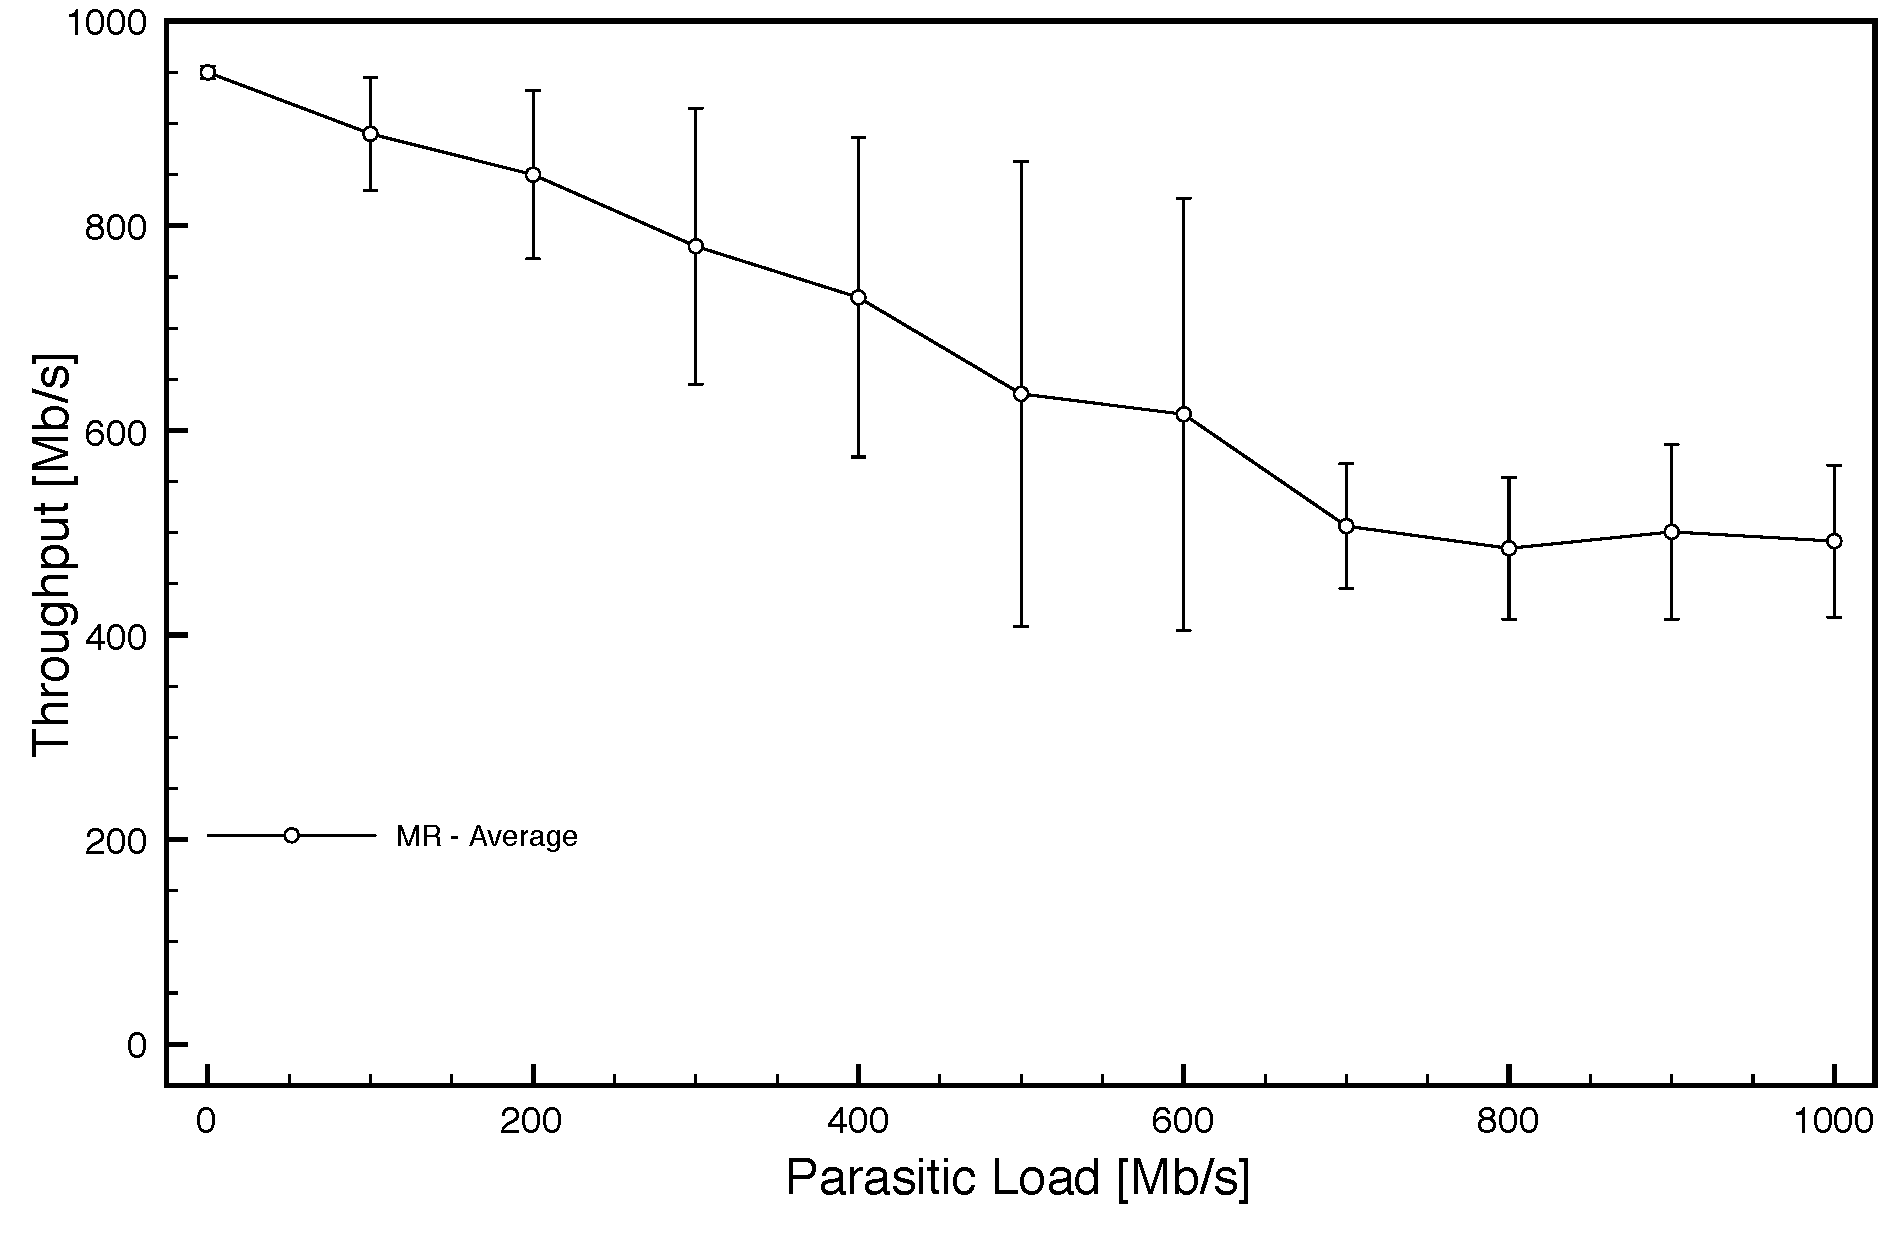
\includegraphics[scale=0.38]{Flower/PDF/MRVar}} 
  
  \subfloat[Hash Threshold's throughput variation]{\label{fig:MRvsHTEb}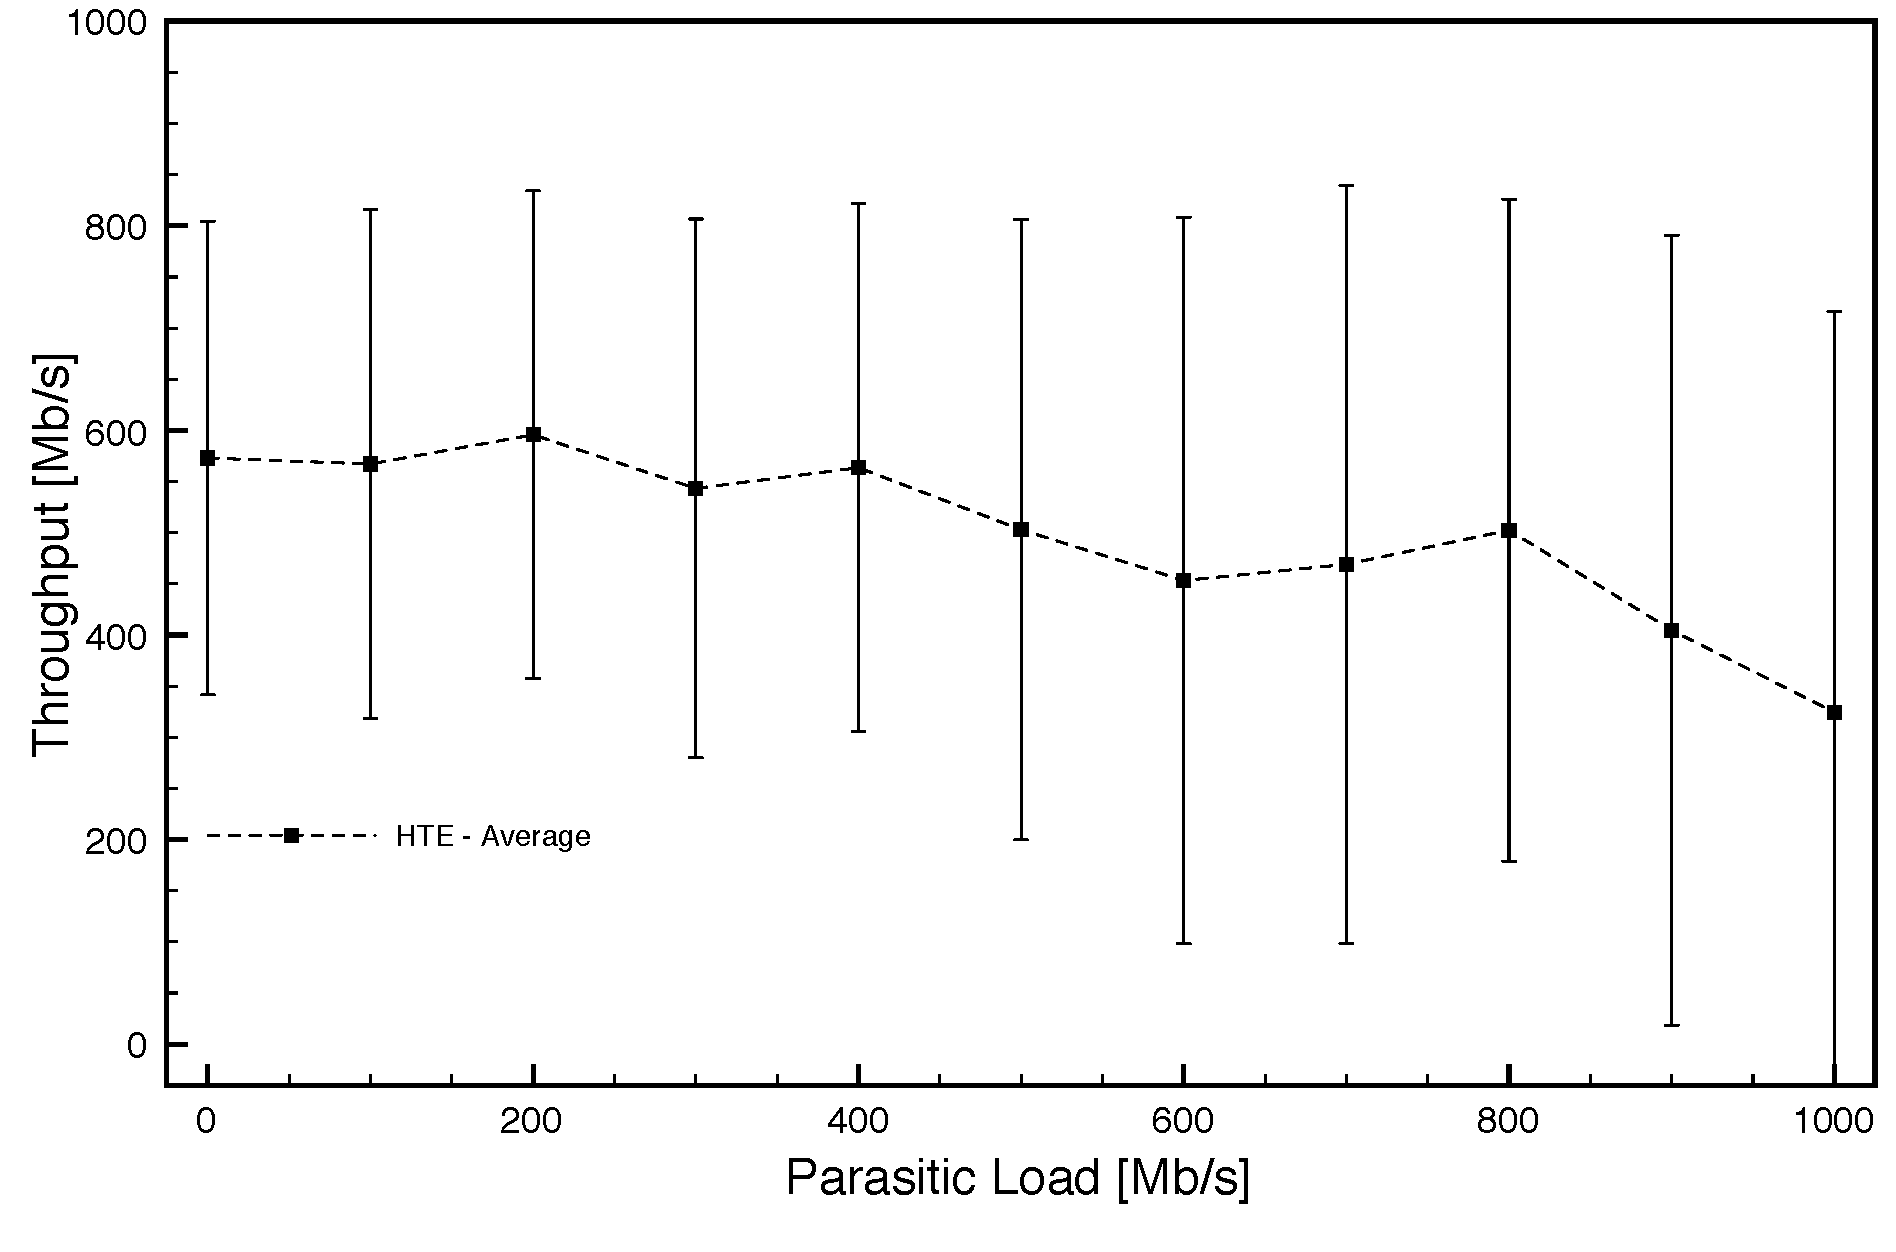
\includegraphics[scale=0.38]{Flower/PDF/HTEVar}}
  \caption{A comparison of the predictability of MultiRoute versus Hash Threshold}
  \label{fig:MRvsHTEFlower}
\end{figure}

Figure \ref{fig:MRvsHTEFlower} shows the average throughput with error bars which represent the variation in throughput observed when running our tests for MultiRoute (Figure \ref{fig:MRvsHTEa}) and HTE (Figure \ref{fig:MRvsHTEb}) . These measurements where done while varying the parasitic traffic rate. Considering only the result for HTE, we observe a large variation of minimum and maximum values. This is explained by the fact that HTE does not consider congestion statistics, and therefore flows may in one case share links and not in others. This phenomenon is especially apparent when the parasitic traffic is high, in some cases all flows will share the same path as the parasitic traffic, causing quasi null throughput for these flows, and in others one flow will be alone on an uncongested path resulting in line rate throughput. These results show that in such situations, HTE throughput can become difficult or nearly impossible to predict accurately. Consider now the results for MultiRoute, the variance between the maximum and minimum values is significantly smaller than in the case of HTE, especially when the parasitic traffic is high. As the parasitic traffic increases in intensity, MultiRoute will route all TCP flows onto the same path causing, like in Figure \ref{fig:MRvsSPFlower}, to share the available bandwidth while avoiding the path used by the parasitic traffic.These results show that we can predict with a significantly higher degree of confidence the expected throughput of MultiRoute in the presence of other traffic flows. It is also interesting to notice than in average MultiRoute performs better than HTE.

\subsection{Parasite Traffic on the Pentagon}

In this setup, parasitic UDP traffic is sent from SW2 to SW5 via SW6. Then, two TCP flows are sent along that same path. 

\subsubsection{Shortest Path versus MultiRoute}

In this situation, there is more than one alternative path to the destination. Therefore, it is expected that all the congestion aware protocols will eventually use all the available paths and therefore avoid the parasitic traffic altogether. Indeed, as we can see in Figure \ref{fig:MRvsSPPentagon}, one TCP flow shares the shortest path to the destination with the parasitic traffic but then switches to an alternative path when the shortest path is marked as congested.  

\ifigure{Pentagon/PDF/MRvsSP}{.38}{Shortest Path versus MultiRoute in the presence of Parasitic Traffic.}{fig:MRvsSPPentagon}

\subsubsection{Shortest Path versus StepRoute}

When running this test with StepRoute, we observe the same behavior except that both TCP flows quickly run at line rate as can be seen in Figure \ref{fig:SRvsSPPentagon}. This can easily be explained by the fact that StepRoute uses congestion classes and not a single bit only. Therefore, as StepRoute quickly marks the link used by the parasitic traffic as lightly congested, it directly uses the alternative path to the destination. We can therefore say that StepRoute is quite sensitive to the congestion status of the various paths. 

\ifigure{Pentagon/PDF/SRvsSP}{.38}{Shortest Path versus StepRoute in the presence of Parasitic Traffic.}{fig:SRvsSPPentagon}

\subsubsection{Shortest Path versus PathRoute}

Figure \ref{fig:PRvsSPPentagon} shows the same test when running PathRoute. Since MultiRoute and PathRoute use the same mechanism to detect and represent congestion we observe a similar result to the one presented in Figure \ref{fig:MRvsSPPentagon} with MultiRoute. But the performance of PathRoute is significantly lower than  MultiRoute or StepRoute. This can be explained due to the longer feedback loop which is introduced by PathRoute's complexity (ie. the knowledge of congestion for a source to any destination). The long feedback loop causes PathRoute to take decisions which are out of sync with the current network status.

\ifigure{Pentagon/PDF/PRvsSP}{.38}{Shortest Path versus PathRoute in the presence of Parasitic Traffic.}{fig:PRvsSPPentagon}

\section{Fully-Meshed Traffic}

Fully-Meshed traffic is the worst possible situation for our protocols as they represent conditions where congestion is equal and omnipresent throughout the network. These tests were performed using the GETB boards. Four end nodes were connected to each switch then each end node sends traffic to each other end node at varying loads from 1\% to 25\% (as this sums up to 100\% for each switch) and the behavior of each protocol is observed. 

For both topologies, one might expect to see a linear throughput until some asymptotic limit, but this is not what was observed in either case. This can be explained by the fact that effective throughput is essentially a function of a switch's packet drop probability. The higher this probability is, the lower the throughput will be. Therefore, when traffic is run through one switch we observe linear increase in throughput as the load increases, because the drop probability is a linear function of the load. Unfortunately this is not the case when there are multiple switches connected to each other. Indeed, while the packet drop probability is still a function of the load, it is now also conditional on the packet drop probability of the previous switch. This conditional probability manifests itself in the following plots as variations (or ``kinks'') in the measured throughput curves.

An attempt was made at modeling this conditional probability using Bayesian Networks \cite{BayesNetwork}, but the model turned out to be vastly too complex and resulted in a combinatorial explosion for the expression of this probability.

%\newpage

\subsection{Fully-Meshed Traffic on the Flower}

\ifigure{Flower/PDF/FullMesh}{.35}{Fully-Meshed Traffic running on the Flower.}{fig:FMFlower}

As is shown in Figure \ref{fig:FMFlower}, all the protocols seem to perform similarly. We can explain this by the fact that all the paths are congested and therefore our congestion aware protocols quickly default to the shortest path. That said, there is a slight (albeit marginal) increase in performance for our protocols. This increase in performance can be better observed when the tests are run successively in order to eliminate the effect of the variations in the throughput as shown in Figure \ref{fig:FMFlowerProbable}. We observe that even though the throughput for both protocols is similar, we clearly notice that as the load increases the difference in the throughput between the shortest path protocol and the congestion-aware increases in average. Actually, there is about a 2GB difference on average, this equates to roughly 66MB every second which means that our protocols have added $\frac{2}{3}$ of a Gigabit link over a shortest path protocol. We believe that this a significant achievement in a Fully-Meshed environment.

\ifigure{Flower/PDF/ProbableLosses}{.38}{Successive Fully-Meshed Traffic running on the Flower.}{fig:FMFlowerProbable}

\subsection{Fully-Meshed Traffic on the Pentagon}

In a topology which offers more alternative paths, we clearly see that our protocols consistently outperform legacy protocols. It is particularly interesting to observe that the Hash Threshold variant of ECMP performs least well. We can explain this by the  manner in which HTE selects its next-hop (based on the source and destination MAC addresses), source-destination pairs will always use the same path regardless of the load they impose on the network and therefore not only does HTE overload those paths it also uses longer congested paths to the destination which significantly decreases its performance.


\ifigure{Pentagon/PDF/FullMesh}{.38}{Fully-Meshed Traffic running on the Pentagon.}{fig:FMPentagon}

\section{Latency \& Packet Loss Tests}

These final results were also obtained using the GETB boards. Full-Mesh traffic was run on each topology, then a stream of probe traffic was sent between two nodes on the network. The time of arrival of the probe traffic as measured and the number of packets lost was counted.

Before explaining the results in this section, we should comment the pseudo step function that is observed in both latency plots below. The linear part of the curve can be seen as the buffers at a router filling, once full we see a significant increase in latency as the switch requires more time to let a packet through its full buffers. From the theory we would expect a linear increase as the router buffers fill up followed by a flat line when all the buffers are full. Unfortunately, this is where our theory and practice differ as it is mathematically complex to construct a queuing model which can tolerate losses. If we consider a single router situation we would observe a linear increase followed by a flatline as the buffers start to drop packets. But now, as we have several routers in a row, we observe a step function which is explained by the fact that a router who is dropping packets has an influence on the loss probability of the next router in the chain who now has a lower loss rate due to a lighter input. Hence, we observe a step function as the routers in the chain have differing rates of buffer saturation.

\subsection{Latency \& Packet loss on the Flower}

\ifigure{Flower/PDF/Latency}{.3}{Latency plots for protocols running on the Flower.}{fig:FlowerLatency}

\ifigure{Flower/PDF/PacketLoss}{.3}{Packet Loss for protocols running on the Flower.}{fig:FlowerPacketLoss}

Figures \ref{fig:FlowerLatency} and \ref{fig:FlowerPacketLoss} show the latency and packet loss experienced by the different protocols respectively. In the case of latency we can see that our protocols present paths which provide less latency, which is to be expected because in this topology we have alternative paths of identical lengths and therefore our latency should either be equal to the shortest path or less. For packet loss, we see that both MultiRoute and StepRoute perform better than the other protocols, this is consistent with our previous results (see Figure \ref{fig:FMFlower}) as they present increased performance in terms of throughput. On the other hand PathRoute performs less well, but again this is consistent as PathRoute does not perform well in terms of throughput during a full-mesh.

\subsection{Latency \& Packet loss on the Pentagon}

\ifigure{Pentagon/PDF/Latency}{.3}{Latency plots for protocols running on the Pentagon.}{fig:PentagonLatency}

\ifigure{Pentagon/PDF/PacketLoss}{.3}{Packet Loss for protocols running on the Pentagon.}{fig:PentagonPacketLoss}

In this case, it is interesting to see that protocols, namely MultiRoute and StepRoute, present a higher latency as shown in Figure \ref{fig:PentagonLatency}. We can explain this by simply noticing that the alternative paths for this topology are longer that the shortest path and therefore require a higher transit time. Figure \ref{fig:PentagonPacketLoss} confirms this observation as the packet loss presented by StepRoute and MultiRoute is lower than the Shortest Path protocol, which means that an alternative path must have been used else the packet loss would have been similar to the shortest path.

\section{Summary}

As these results have shown, our congestion-aware protocols have outperformed legacy protocols. Both, in worst case situations (Full-Mesh) and rather advantageous positions (Parasitic Traffic). Nevertheless, deployment of such protocols requires a rigorous study of the type of services which will de offered by the network. For example, if a network is supposed to carry mainly Voice-over-IP traffic then the network engineer should make sure to provide paths of identical lengths to all destinations in an effort to keep the traffic latencies constant. 

Naively, one would expect that a protocol which has quasi network wide knowledge, such as PathRoute, would deliver optimal results. Unfortunately this is not the case, from the results presented in this chapter we clearly observe that PathRoute performs significantly worse than its peers (MultiRoute and StepRoute). This phenomenon is exacerbated when we consider fullmesh situations. The reason for this lack in performance can be found in control theory's standard problem, ie. the duration on the feedback loop. While all the congestion-aware routing protocols presented in this thesis suffer from a delay between observing congestion and adapting the network state to reflect this change, the impact on PathRoute is more significant that on its peers. Indeed, any update in any area of the network may, in the worst case, trigger updates at all the routers in the network and therefore cause some routers to have opposing network views thereby causing poor routing decisions to be taken.

%Another, rather disappointing, observation is that  PathRoute did not perform as well as we would have liked (or indeed expected). The explanation lies within that fact that PathRoute requires a relatively large amount of signaling and that it assumes that updates from routers which lie on a path  from a source to a destination are synchronous. This assumption does not hold in PathRoute current implementation as each transfer function is independent of one another and therefore segments of a path may report different congestion states and thus cause source routers to make incorrect routing decisions. A rather simple solution to this would be add an extra layer of signaling for PathRoute, but this could prove to be expensive and may impact the reactivity of the protocol.